% Options for packages loaded elsewhere
\PassOptionsToPackage{unicode}{hyperref}
\PassOptionsToPackage{hyphens}{url}
\PassOptionsToPackage{dvipsnames,svgnames,x11names}{xcolor}
%
\documentclass[
  letterpaper,
  DIV=11,
  numbers=noendperiod]{scrartcl}

\usepackage{amsmath,amssymb}
\usepackage{iftex}
\ifPDFTeX
  \usepackage[T1]{fontenc}
  \usepackage[utf8]{inputenc}
  \usepackage{textcomp} % provide euro and other symbols
\else % if luatex or xetex
  \usepackage{unicode-math}
  \defaultfontfeatures{Scale=MatchLowercase}
  \defaultfontfeatures[\rmfamily]{Ligatures=TeX,Scale=1}
\fi
\usepackage{lmodern}
\ifPDFTeX\else  
    % xetex/luatex font selection
\fi
% Use upquote if available, for straight quotes in verbatim environments
\IfFileExists{upquote.sty}{\usepackage{upquote}}{}
\IfFileExists{microtype.sty}{% use microtype if available
  \usepackage[]{microtype}
  \UseMicrotypeSet[protrusion]{basicmath} % disable protrusion for tt fonts
}{}
\makeatletter
\@ifundefined{KOMAClassName}{% if non-KOMA class
  \IfFileExists{parskip.sty}{%
    \usepackage{parskip}
  }{% else
    \setlength{\parindent}{0pt}
    \setlength{\parskip}{6pt plus 2pt minus 1pt}}
}{% if KOMA class
  \KOMAoptions{parskip=half}}
\makeatother
\usepackage{xcolor}
\setlength{\emergencystretch}{3em} % prevent overfull lines
\setcounter{secnumdepth}{-\maxdimen} % remove section numbering
% Make \paragraph and \subparagraph free-standing
\ifx\paragraph\undefined\else
  \let\oldparagraph\paragraph
  \renewcommand{\paragraph}[1]{\oldparagraph{#1}\mbox{}}
\fi
\ifx\subparagraph\undefined\else
  \let\oldsubparagraph\subparagraph
  \renewcommand{\subparagraph}[1]{\oldsubparagraph{#1}\mbox{}}
\fi


\providecommand{\tightlist}{%
  \setlength{\itemsep}{0pt}\setlength{\parskip}{0pt}}\usepackage{longtable,booktabs,array}
\usepackage{calc} % for calculating minipage widths
% Correct order of tables after \paragraph or \subparagraph
\usepackage{etoolbox}
\makeatletter
\patchcmd\longtable{\par}{\if@noskipsec\mbox{}\fi\par}{}{}
\makeatother
% Allow footnotes in longtable head/foot
\IfFileExists{footnotehyper.sty}{\usepackage{footnotehyper}}{\usepackage{footnote}}
\makesavenoteenv{longtable}
\usepackage{graphicx}
\makeatletter
\def\maxwidth{\ifdim\Gin@nat@width>\linewidth\linewidth\else\Gin@nat@width\fi}
\def\maxheight{\ifdim\Gin@nat@height>\textheight\textheight\else\Gin@nat@height\fi}
\makeatother
% Scale images if necessary, so that they will not overflow the page
% margins by default, and it is still possible to overwrite the defaults
% using explicit options in \includegraphics[width, height, ...]{}
\setkeys{Gin}{width=\maxwidth,height=\maxheight,keepaspectratio}
% Set default figure placement to htbp
\makeatletter
\def\fps@figure{htbp}
\makeatother

\KOMAoption{captions}{tableheading}
\makeatletter
\@ifpackageloaded{caption}{}{\usepackage{caption}}
\AtBeginDocument{%
\ifdefined\contentsname
  \renewcommand*\contentsname{Table of contents}
\else
  \newcommand\contentsname{Table of contents}
\fi
\ifdefined\listfigurename
  \renewcommand*\listfigurename{List of Figures}
\else
  \newcommand\listfigurename{List of Figures}
\fi
\ifdefined\listtablename
  \renewcommand*\listtablename{List of Tables}
\else
  \newcommand\listtablename{List of Tables}
\fi
\ifdefined\figurename
  \renewcommand*\figurename{Figure}
\else
  \newcommand\figurename{Figure}
\fi
\ifdefined\tablename
  \renewcommand*\tablename{Table}
\else
  \newcommand\tablename{Table}
\fi
}
\@ifpackageloaded{float}{}{\usepackage{float}}
\floatstyle{ruled}
\@ifundefined{c@chapter}{\newfloat{codelisting}{h}{lop}}{\newfloat{codelisting}{h}{lop}[chapter]}
\floatname{codelisting}{Listing}
\newcommand*\listoflistings{\listof{codelisting}{List of Listings}}
\makeatother
\makeatletter
\makeatother
\makeatletter
\@ifpackageloaded{caption}{}{\usepackage{caption}}
\@ifpackageloaded{subcaption}{}{\usepackage{subcaption}}
\makeatother
\ifLuaTeX
  \usepackage{selnolig}  % disable illegal ligatures
\fi
\usepackage[]{natbib}
\bibliographystyle{plainnat}
\IfFileExists{bookmark.sty}{\usepackage{bookmark}}{\usepackage{hyperref}}
\IfFileExists{xurl.sty}{\usepackage{xurl}}{} % add URL line breaks if available
\urlstyle{same} % disable monospaced font for URLs
\hypersetup{
  colorlinks=true,
  linkcolor={blue},
  filecolor={Maroon},
  citecolor={Blue},
  urlcolor={Blue},
  pdfcreator={LaTeX via pandoc}}

\author{}
\date{}

\begin{document}

\subsubsection{Dataset, spacecraft instruments, and solar wind
model}\label{dataset-spacecraft-instruments-and-solar-wind-model}

Synergistic observations \citep{velli2020} advance our understanding of
the solar wind.

\paragraph{Juno}\label{juno}

We use the following data collected by Juno: magnetic fields with a ∼1s
resolution by the Juno Fluxgate Magnetometer (MAG)
\citep{connerney2017}, the ion bulk velocity \(v\), and the plasma
density \(n\) with a hourly resolution from solar wind model (see
below).

\paragraph{Parker Solar Probe (PSP)}\label{parker-solar-probe-psp}

We use the following data collected by PSP: magnetic fields by the FIELDS
experiment \citep{bale2016}, the ion bulk velocity \(v\), and the plasma
density \(n\) with a hourly resolution by the Solar Wind Electrons
Alphas and Protons (SWEAP) Investigation \citep{kasper2016}.

\paragraph{ARTEMIS}\label{artemis}

We use the following data collected by ARTEMIS: magnetic fields with a
∼1s resolution by the Fluxgate Magnetometer \citep{auster2008}, the ion
bulk velocity \(v\), and the plasma density \(n\) calculated from
velocity distribution by the Electrostatic Analyzer
\citep{mcfadden2009}.

\paragraph{STEREO}\label{stereo}

We use the following data collected by STEREO: magnetic fields with a
∼1/8 s resolution by the magnetic field experiment \citep{acuña2008} on
In-situ Measurements of Particles and CME Transients (IMPACT)
\citep{luhmann2008}, the ion bulk velocity \(v\), and the plasma density
\(n\) with a hourly resolution by the Plasma and Suprathermal Ion
Composition (PLASTIC) \citep{galvin2008}.

\paragraph{Wind}\label{wind}

We use the following data collected by Wind: magnetic fields with a ∼1/11
s resolution by the Magnetic Field Investigation (MFI)
\citep{lepping1995}, the ion bulk velocity \(v\), and the plasma density
\(n\) with a hourly resolution by the Solar Wind Experiment (SWE)
\citep{ogilvie1995}.

\paragraph{Solar wind model}\label{solar-wind-model}

The hourly solar wind model data from the Two-Dimensional Outer
Heliosphere Solar Wind Modeling (MSWIM2D) \citep{keebler2022} were
employed to determine the ion bulk velocity \(v\) and plasma density
\(n\) at the location of the Juno mission. Utilizing the BATSRUS MHD
solver, this model is capable of simulating the propagation of the solar
wind from 1 to 75 astronomical units (AU) in the ecliptic plane,
effectively encompassing the region of interest for our study.

\begin{figure}[H]

{\centering 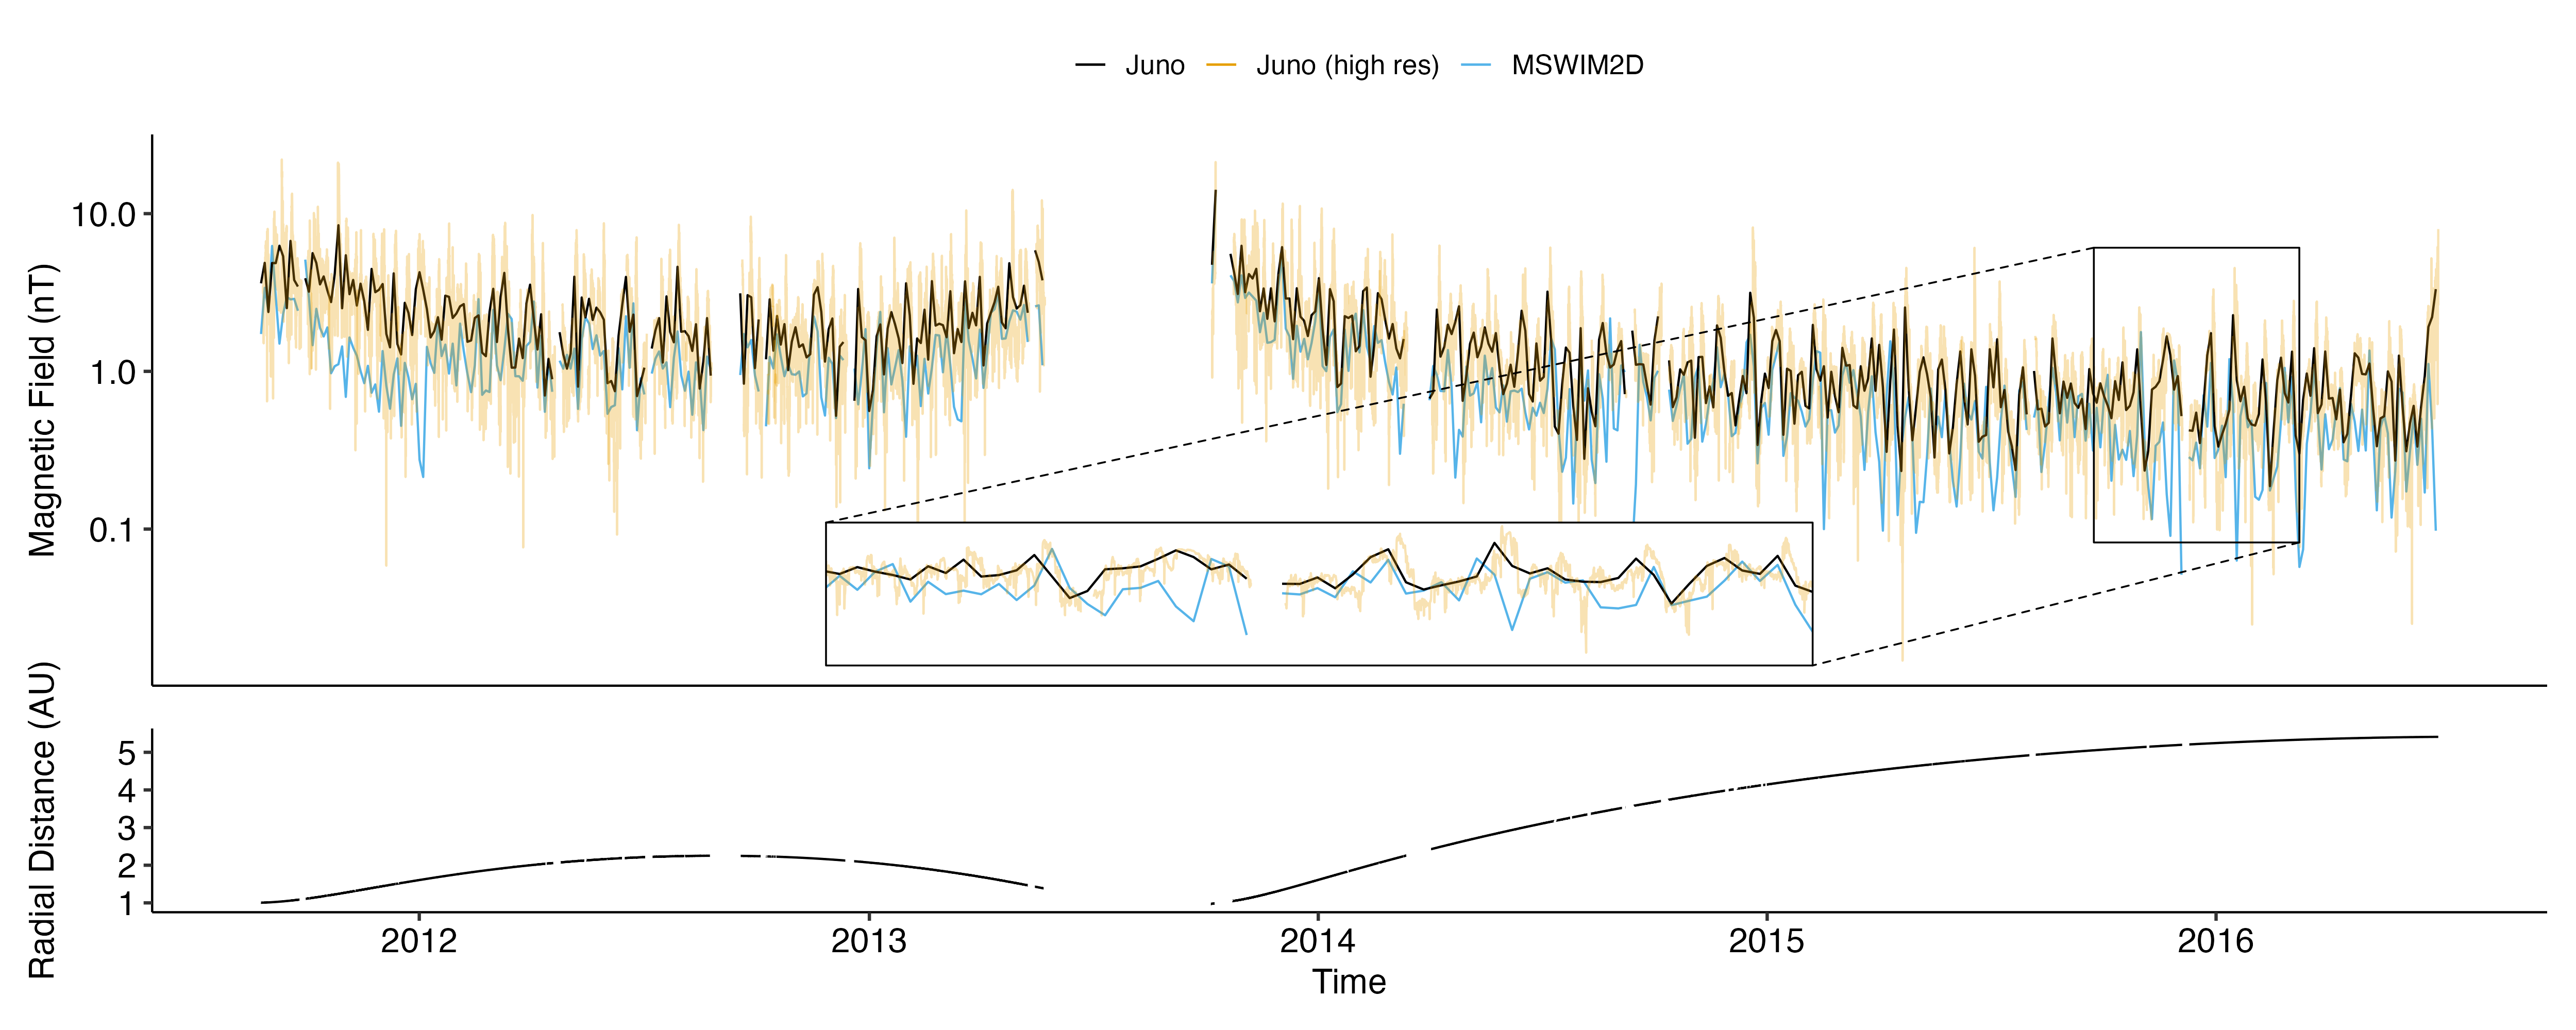
\includegraphics{images/juno_model_validation.png}

}

\caption{Time-series comparison of MSWIM2D (red) and Juno-observed solar
wind}

\end{figure}%

\subsubsection{Determination of
discontinuities}\label{determination-of-discontinuities}

We use \citep{liu2022a} method to identify IDs, which has better
compatibility for the IDs with minor field changes, and is more robust
to the situtaion encountered in the outer heliosphere.

In Liu's method : The first two conditions guarantee that the field
changes of the IDs identified are large enough to be distinguished from
the stochastic fluctuations on magnetic fields, while the third is a
supplementary condition to reduce the uncertainty of recognition.

\begin{figure}[H]

{\centering \includegraphics{images/fig-examples.pdf}

}

\caption{Rotational discontinuities (RDs) detected by PSP, Juno, Stereo
and near-Earth satellite at different radial distances and solar
longitudes.}

\end{figure}%


  \bibliography{files/references.bib}


\end{document}
